\documentclass[twocolumn, 10pt]{article} % 全局字体大小设为12pt

% 导入 ctex 包以支持中文
\usepackage[UTF8]{ctex}
\usepackage{courier} % 用于设置代码字体

% 设置页面边距
\usepackage{geometry}
\geometry{left=2cm,right=2cm,top=2.5cm,bottom=2.5cm}
\usepackage{amsthm}

\usepackage{listings} % 用于显示代码
\usepackage{color}

% 自定义带编号且斜体内容的 remark 环境
\theoremstyle{remark}
\newtheorem{remark}{Remark}

% 通过\textit命令让内容显示为斜体
\newenvironment{myremark}
  {\begin{remark}\itshape}
  {\end{remark}}


% 其他常用包
\usepackage{graphicx}   % 插入图片
\usepackage{amsmath}    % 数学公式
\usepackage{amssymb}    % 数学符号
\usepackage{hyperref}   % 超链接
\usepackage{enumitem}   % 引入 enumitem 包用于自定义列表
\usepackage{array} % 提供表格增强功能
\usepackage{stfloats} % 支持双栏排版中的浮动对象

\usepackage{hyperref}

\usepackage{xcolor} % 用于设置文本和背景颜色
\usepackage{times} % 设置全局字体为 Times New Roman,或者根据需求选择其他字体
% 表格字体设置
\usepackage{etoolbox}

% 导入titlecaps宏包
\usepackage{titlecaps}

\definecolor{codegray}{rgb}{0.5,0.5,0.5}
\definecolor{codeblue}{rgb}{0.25,0.5,0.75}
\definecolor{codepurple}{rgb}{0.58,0,0.82}

\lstdefinestyle{mystyle}{
    backgroundcolor=\color{white},   
    commentstyle=\color{codegray},
    keywordstyle=\color{codeblue},
    numberstyle=\tiny\color{codegray},
    stringstyle=\color{codepurple},
    basicstyle=\ttfamily\scriptsize, % 调整代码字体大小为 \scriptsize
    breakatwhitespace=false,         
    breaklines=true,                 
    captionpos=b,                    
    keepspaces=true,                 
    numbers=left,                    
    numbersep=5pt,                  
    showspaces=false,                
    showstringspaces=false,
    showtabs=false,                  
    tabsize=2
}

\lstset{style=mystyle}


% 自定义命令将标题首字母大写,其他单词小写
\Addlcwords{a an the of and in on at to with by for from}
\newcommand{\capitalizeTitle}[1]{\titlecap{#1}}

% 设置标题格式
\usepackage{titlesec}
\titleformat{\section}
  {\normalfont\Large\bfseries}
  {\thesection}{1em}{\capitalizeTitle}

\titleformat{\subsection}
  {\normalfont\large\bfseries}
  {\thesubsection}{1em}{\capitalizeTitle}

\titleformat{\subsubsection}
  {\normalfont\normalsize\bfseries}
  {\thesubsubsection}{1em}{\capitalizeTitle}









\AtBeginEnvironment{tabular}{\small} % 将表格内字体设为比正文小1号


% 定义浅黄色
\definecolor{lightyellow}{rgb}{1.0, 1.0, 0.88}

\begin{document}

% 标题
\title{Mastering LLM Techniques Inference Optimization}
\author{https://developer.nvidia.com/blog/mastering-llm-techniques-inference-optimization/}
\date{\today}
\maketitle
% 摘要


\section{理解LLM推理}

将变压器层叠加在一起以创建大型模型,可以提高准确性、少样本学习能力,甚至在广泛的语言任务中表现出接近人类的涌现能力。这些基础模型的训练成本高昂,在推理过程中(一个持续的成本)也可能消耗大量的内存和计算资源。目前最流行的大语言模型(LLM)参数规模可达到数百亿,根据具体使用场景,可能需要处理长输入,这也会增加开销。例如,检索增强生成(RAG)管道需要将大量信息输入模型,极大地增加了LLM的处理工作量。

本文讨论了LLM推理中最紧迫的挑战及一些实用的解决方案。读者应对变压器架构和注意力机制有基本的理解。掌握LLM推理的复杂性非常重要,这将在下一节中详细探讨。

\section{Understanding LLM inference}

大多数流行的仅解码器大语言模型(如GPT-3)在因果建模目标上进行预训练,主要作为下一个词的预测器。这些LLM将一系列词元作为输入,自回归地生成后续词元,直到满足停止标准(例如生成词元的数量限制或停用词列表),或生成标记生成结束的特殊\texttt{<end>}词元。这个过程包括两个阶段:预填充阶段和解码阶段。

需要注意的是,词元是模型处理语言的基本单位。一个词元大约等于四个英文字符。所有自然语言的输入在输入模型之前都会被转换为词元。

\subsection{Prefill phase or processing the input}
在预填充阶段,LLM处理输入的词元以计算中间状态(键和值),这些状态用于生成“第一个”新词元。每个新词元都依赖于所有之前的词元,但由于输入的整体范围已知,从高层次来看,这实际上是一个高度并行的矩阵运算。这个过程有效地最大化了GPU的利用率。

\subsection{Decode phase or generating the output}
在解码阶段,LLM通过自回归方式一次生成一个输出词元,直到满足停止条件。每个顺序输出的词元都需要了解之前所有迭代的输出状态(键和值)。与预填充阶段相比,这类似于矩阵-向量操作,GPU的计算能力未得到充分利用。此过程的延迟主要由数据(权重、键、值、激活)从内存传输到GPU的速度决定,而非计算速度。因此,这是一个受内存限制的操作。

\textbf{本文中的许多推理挑战和相应的解决方案都涉及解码阶段的优化:高效的注意力模块、有效管理键和值等。}

不同的LLM可能使用不同的分词器,因此在它们之间比较输出词元可能并不简单。即使两个LLM的每秒输出词元数相似,如果使用不同的分词器,它们可能并不等效,因为相应的词元可能代表不同数量的字符。




\subsection{Batching}
提高GPU利用率和吞吐量的最简单方法是通过批处理。由于多个请求使用相同的模型,权重的内存成本得以分摊。将更大的批次同时传输到GPU处理可以更好地利用可用的计算资源。

然而,批次大小只能增加到一定限度,超出后可能导致内存溢出。为更好地理解这一点,需要研究键值(KV)缓存和LLM的内存需求。

传统的批处理(也称为静态批处理)效果不佳,因为批次中的每个请求可能生成不同数量的完成词元,导致执行时间不同。结果是所有请求必须等到最长的请求完成,这种情况可能因生成长度的差异而加剧。可以通过一些方法来缓解这一问题,例如后续将讨论的“在途批处理”(in-flight batching)。

\subsection{Key-value caching}
\begin{figure*}[ht]
    \centering
    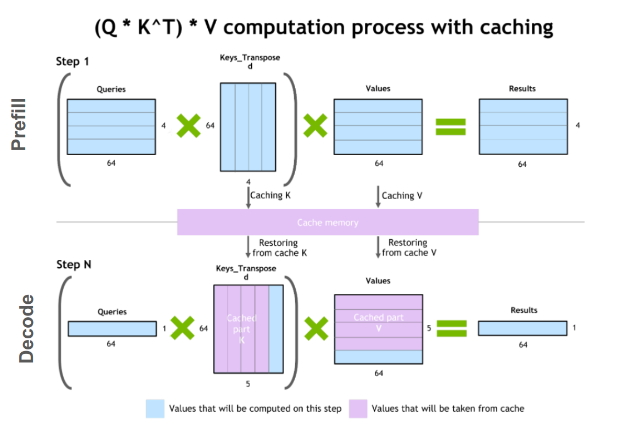
\includegraphics[width=0.8\textwidth]{key-value-caching_.png}
    \caption{Key-Value Caching 示意图}
\end{figure*}


解码阶段的一个常见优化方法是键值(KV)缓存。解码阶段在每个时间步生成一个词元,但每个词元都依赖于之前所有词元的键和值张量(包括在预填充阶段计算的输入词元的KV张量,以及直到当前时间步计算出的任何新KV张量)。

为了避免在每个时间步重新计算所有这些张量,可以将它们缓存到GPU内存中。每次迭代时,新元素被计算出来后,简单地添加到现有缓存中,以便在下一个迭代中使用。在某些实现中,每一层模型都有一个KV缓存。



\section{LLM memory requirement }


实际上,GPU LLM内存需求的两个主要因素是模型权重和KV缓存。

\subsection{模型权重}
内存被模型参数占用。例如,一个具有70亿参数的模型(如Llama 2 7B),加载为16位精度(FP16或BF16)时,大约需要7B * sizeof(FP16) ≈ 14 GB的内存。

\subsection{KV缓存}
内存被自注意力张量的缓存占用,以避免重复计算。在批处理情况下,批次中每个请求的KV缓存仍需分别分配,并且可能占用大量内存。下列公式描述了KV缓存的大小,适用于当今最常见的LLM架构。

每个词元的KV缓存大小(字节) = 2 * (层数) * (头数 * 头维度) * 精度字节数

第一个系数2代表K和V矩阵。通常情况下,(头数 * 头维度)的值与变压器的隐藏层大小(或模型维度,d\_model)相同。这些模型属性通常可以在模型卡或相关配置文件中找到。

对于输入序列中的每个词元,这个内存大小是跨批次输入所需的。假设半精度,总KV缓存大小由以下公式给出。

KV缓存总大小(字节)= (批次大小) * (序列长度) * 2 * (层数) * (隐藏层大小) * sizeof(FP16)

例如,对于一个使用16位精度的Llama 2 7B模型,批次大小为1时,KV缓存的大小将为1 * 4096 * 2 * 32 * 4096 * 2字节,大约为2 GB。

有效管理这个KV缓存是一个具有挑战性的任务。随着批次大小和序列长度的线性增长,内存需求可以迅速扩大。因此,它限制了可提供的吞吐量,并对长上下文输入提出了挑战。这也正是本文中介绍的几种优化方法的动机所在。

\subsection{Scaling up LLMs with model parallelization}
减少每个设备模型权重内存占用的一种方法是将模型分布在多个GPU上。通过分散内存和计算负担,可以运行更大的模型或更大的输入批次。对于需要超过单个设备可用内存的模型,模型并行化是必需的,以便训练或推理,并使训练时间和推理指标(延迟或吞吐量)适合特定的使用场景。模型并行化有多种方式,取决于模型权重的划分方式。

值得注意的是,数据并行性也是常提到的技术之一。在这种方法中,模型权重被复制到多个设备上,并将输入的(全局)批次大小在每个设备上分成微批次。它通过处理更大的批次来减少整体执行时间,但这更多是训练时的优化,与推理阶段的相关性较小。

\subsection{Pipeline parallelism}
\begin{figure*}[ht]
    \centering
    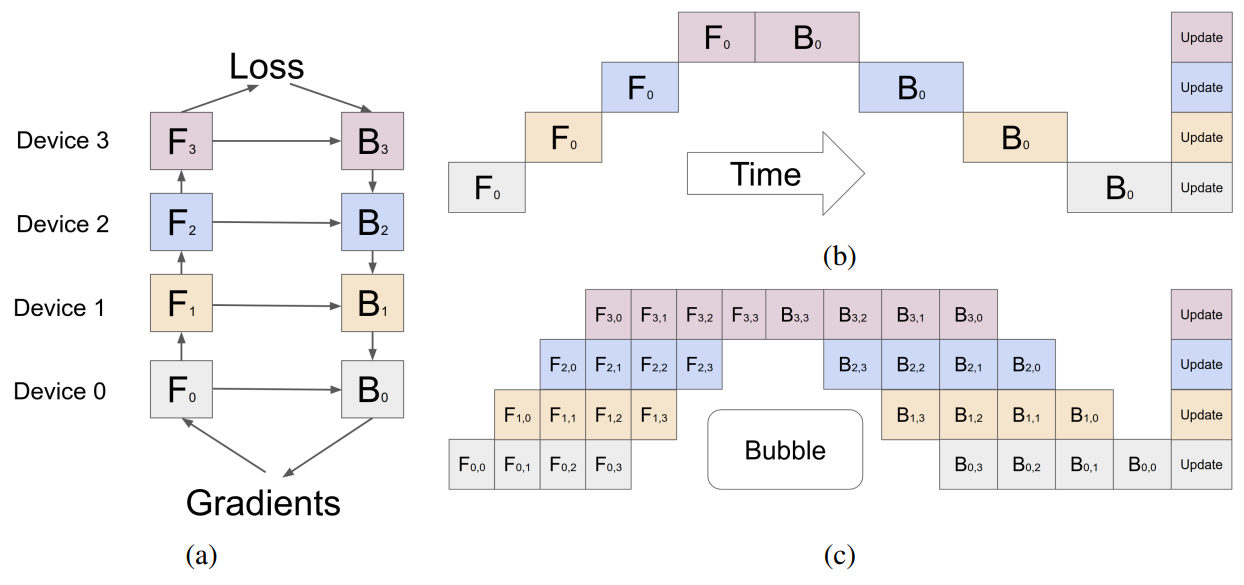
\includegraphics[width=0.8\textwidth]{four-way-pipeline-parallelism.png}
    \caption{An illustration of four-way pipeline parallelism. Credit: GPipe: Easy Scaling with Micro-Batch Pipeline Parallelism}
\end{figure*}

流水线并行涉及将模型(纵向)划分为多个块,每个块包含在一个独立设备上执行的一部分层。图2a展示了四路流水线并行的示意图,其中模型被顺序划分,每个设备执行四分之一的层。一个设备上的操作组的输出会传递给下一个设备,继续执行后续块。$F_n$和$B_n$分别表示设备n上的前向和反向传递。这样,每个设备上存储模型权重的内存需求被有效减少了四分之三。

这种方法的主要限制是由于处理的顺序性,一些设备或层在等待前一层的输出(激活、梯度)时可能会闲置,导致前向和反向传递中出现效率低下或“流水线气泡”。图2b中,白色空白区域是使用简单流水线并行时出现的大量流水线气泡,此时设备闲置且利用率低下。

微批处理可以在一定程度上缓解这一问题,如图2c所示。全局批次大小被分割成子批次,逐个处理,最终累积梯度。需要注意的是,$F_{n,m}$和$B_{n,m}$分别表示设备n上对微批次m的前向和反向传递。这种方法缩小了流水线气泡的大小,但并不能完全消除它们。



\subsection{Tensor parallelism}
\begin{figure*}[ht]
    \centering
    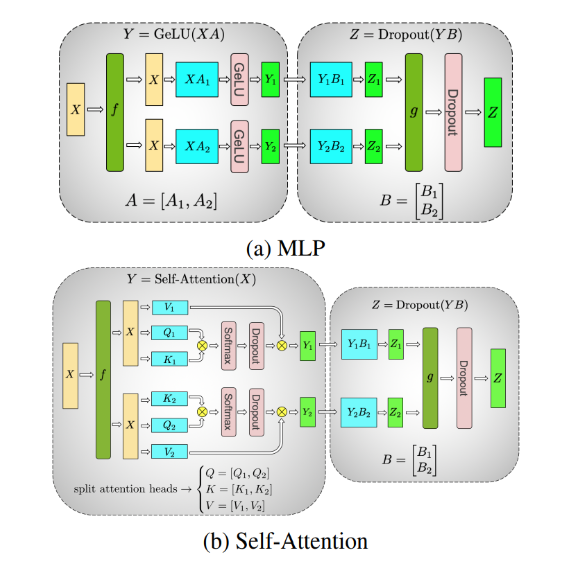
\includegraphics[width=0.8\textwidth]{tensor-parallelsim-mlp-self-attention-layers_.png}
    \caption{Illustration of tensor parallelism in multi-layer perceptron (MLP) and self-attention layers. Credit: Megatron-LM: Training Multi-Billion Parameter Language Models Using Model Parallelism}
\end{figure*}
张量并行涉及将模型的各层(水平)划分为较小的、独立的计算块,这些块可以在不同设备上并行执行。注意力块和多层感知器(MLP)层是变压器的主要组成部分,可以利用张量并行。在多头注意力块中,每个头或头组可以分配到不同的设备上,从而独立并行计算。

图3a展示了在一个两层MLP上的双向张量并行示例,每一层用一个圆角框表示。在第一层中,权重矩阵$A$被分割为$A_1$和$A_2$。计算$XA_1$和$XA_2$可以在两个不同的设备上独立执行,同一批次的输入$X$经过身份操作$f$。这种方法有效地将每个设备上存储权重的内存需求减半。一个归约操作$g$在第二层中将输出合并。


图3b展示了在自注意力层中的双向张量并行示例。多个注意力头本质上是并行的,可以跨设备进行分割。


\subsection{Sequence parallelism}
张量并行有其局限性,因为它要求将层划分为独立的、可管理的块。对于LayerNorm和Dropout等操作,张量并行并不适用,这些操作会在张量并行组中被复制。虽然LayerNorm和Dropout的计算代价较低,但它们确实需要大量内存来存储(冗余的)激活。

如在《Reducing Activation Recomputation in Large Transformer Models》中所示,这些操作在输入序列上是独立的,可以沿着“序列维度”进行分区,使其更具内存效率。这被称为序列并行。

\begin{figure*}[ht]
    \centering
    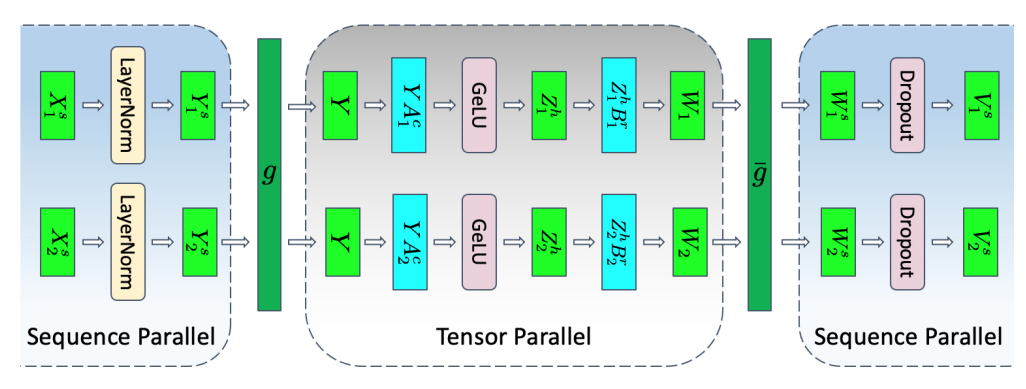
\includegraphics[width=0.8\textwidth]{transformer-layer-tensor-and-sequence-parallelism.png}
    \caption{An illustration of a transformer layer with both tensor and sequence parallelism. Credit: Reducing Activation Recomputation in Large Transformer Models}
\end{figure*}

模型并行技术并不是互斥的,可以结合使用。它们可以帮助扩展和减少每个GPU的LLM内存占用,但也有一些专门针对注意力模块的优化技术。





\section{Optimizing the attention mechanism}


\subsection{Multi-head attention}
\begin{figure*}[ht]
    \centering
    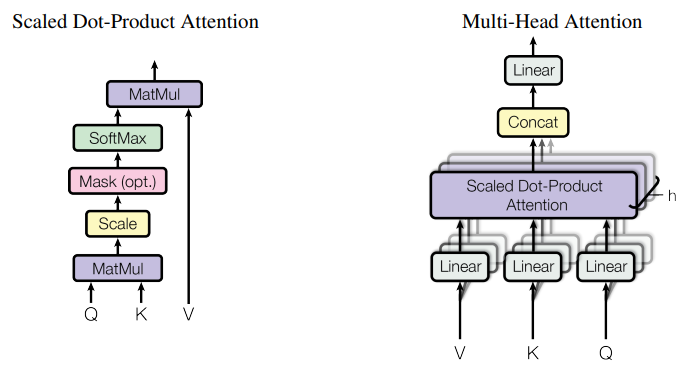
\includegraphics[width=0.8\textwidth]{scaled-dot-product-attention-and-multi-head-attention.png}
    \caption{An illustration of the scaled dot-product attention (left) and multi-head attention (right), which is simply multiple SDPA heads in parallel. Credit: Attention Is All You Need}
\end{figure*}
作为对缩放点积注意力(SDPA)的增强,通过不同的学习投影对Q、K和V矩阵并行多次执行注意力层,使模型能够同时关注输入中不同位置的不同表征子空间的信息。这些子空间独立学习,为模型提供了对输入中不同位置的更丰富理解。

如图5所示,多个并行注意力操作的输出被连接并线性投影以将它们组合。每个并行注意力层称为一个“头”,这种方法被称为多头注意力机制(MHA)。

在最初的研究中,每个注意力头在模型的一个缩小维度上操作(如使用八个平行注意力头时的$d_{model}/8$),这样可以保持计算成本与单头注意力相似。




\subsection{Multi-query attention}


在《Fast Transformer Decoding》中提出的一种针对MHA的推理优化称为多查询注意力(MQA),它在多个注意力头之间共享键和值。查询向量仍然像之前一样进行多次投影。

尽管MQA的计算量与MHA相同,但从内存读取的数据量(键和值)仅为之前的一部分。当受到内存带宽限制时,这可以提高计算利用率。同时,它还减少了内存中KV缓存的大小,为更大的批次大小腾出空间。

减少键值头的数量可能会导致精度下降。此外,需要在推理时利用这种优化的模型必须在启用MQA的情况下进行训练(或至少使用约5\%的训练量进行微调)。



\subsection{Grouped-query attention}

分组查询注意力(GQA)在MHA和MQA之间取得了平衡,它将键和值投影到少数几个查询头组(如图6所示)。在每个组内,GQA的行为类似于多查询注意力。

图6显示了多头注意力(左)有多个键值头;分组查询注意力(中)具有比一个更多但少于查询头数量的键值头,在内存需求和模型质量之间取得平衡;多查询注意力(右)仅有一个键值头,以节省内存。

\begin{figure*}[ht]
    \centering
    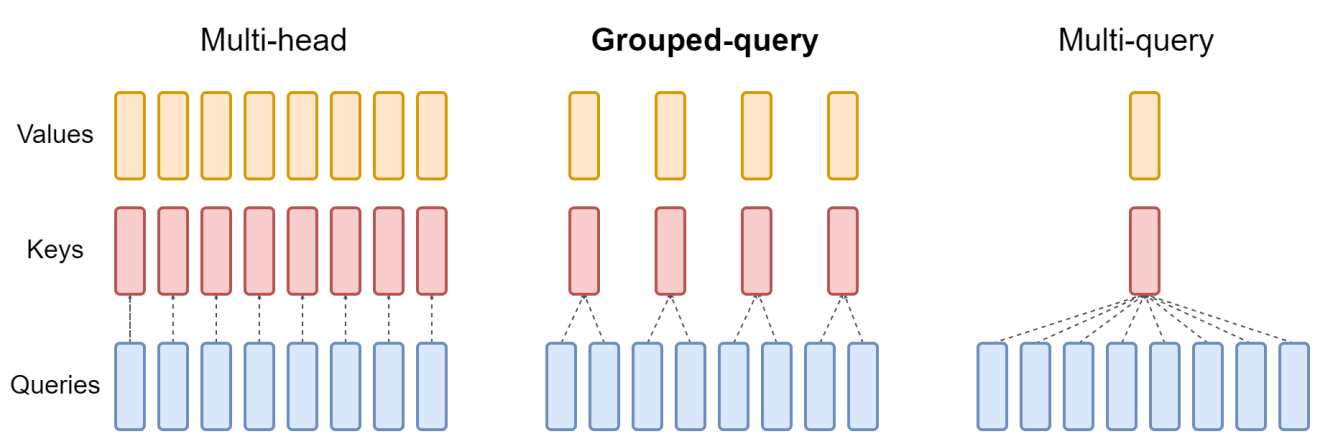
\includegraphics[width=0.8\textwidth]{comparison-attention-mechanisms.png}
    \caption{A comparison of different attention mechanisms. Credit: GQA: Training Generalized Multi-Query Transformer Models from Multi-Head Checkpoints}
\end{figure*}


最初使用MHA训练的模型可以通过使用一小部分原始训练计算量来“升级”到GQA。这些模型在保持接近MQA的计算效率的同时,能够达到接近MHA的质量。Llama 2 70B就是利用GQA的一个例子。

像MQA和GQA这样的优化通过减少存储的键值头的数量来降低KV缓存所需的内存。然而,KV缓存的管理仍可能存在低效。与优化注意力模块本身不同,下一节将介绍一种更高效的KV缓存管理技术。


\section{Flash attention}

\begin{figure*}[ht]
    \centering
    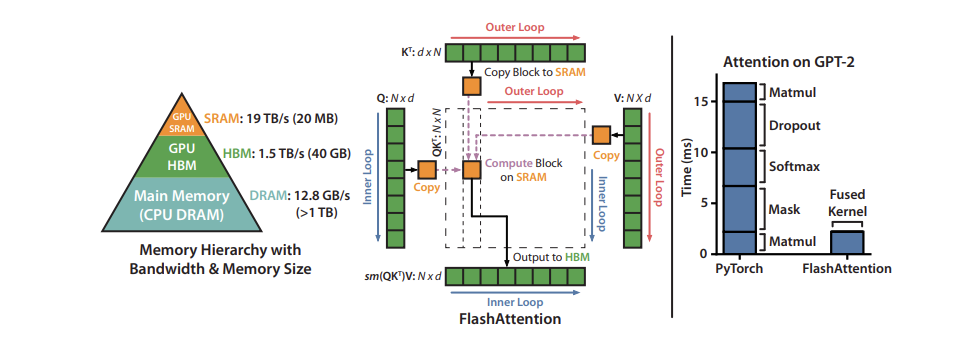
\includegraphics[width=0.8\textwidth]{flash-attention-computation-pattern-memory-hierarchy-gpu.png}
    \caption{The tiled FlashAttention computation pattern and the memory hierarchy on a 40 GB GPU. Credit: FlashAttention: Fast and Memory-Efficient Exact Attention with IO-Awareness}
\end{figure*}


另一种优化注意力机制的方法是修改某些计算的顺序,以更好地利用GPU的内存层次结构。神经网络通常按层次描述,大多数实现也是如此,依次对输入数据进行一种计算。但这并不总是能带来最佳性能,因为对已经加载到更高、更高效内存层次的值进行更多计算可能更有利。

在实际计算过程中,将多个层融合在一起可以最小化GPU从其内存读取和写入的次数,并将需要相同数据的计算组合在一起,即使它们属于神经网络中的不同层次。

一种非常流行的融合方法是FlashAttention,一种I/O感知的精确注意力算法,详细描述见《FlashAttention: Fast and Memory-Efficient Exact Attention with IO-Awareness》。精确注意力意味着它在数学上与标准多头注意力相同(具有适用于多查询和分组查询注意力的变体),因此可以无需修改地替换到现有模型架构或已训练的模型中。

I/O感知意味着它在融合操作时考虑到之前讨论的一些内存移动成本。特别是,FlashAttention使用“平铺”技术一次性完全计算并写出最终矩阵的一小部分,而不是分步骤在整个矩阵上进行部分计算,并在此过程中写出中间值。

图7显示了在40 GB GPU上平铺的FlashAttention计算模式和内存层次结构。右侧的图表显示了通过融合和重新排序注意力机制不同组件所带来的相对加速效果。


\subsection{Efficient management of KV cache with paging}
\begin{figure*}[ht]
    \centering
    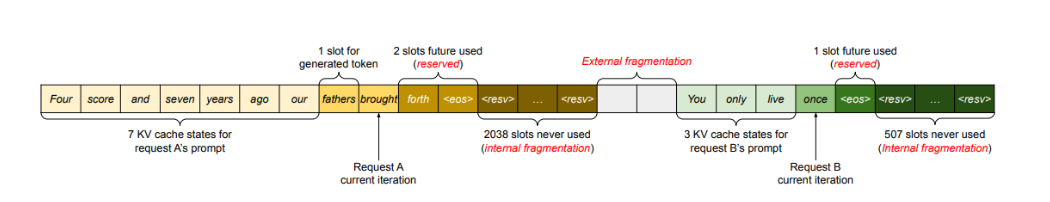
\includegraphics[width=0.8\textwidth]{memory-wastage-fragmentation-inefficient-kv-cache.png}
    \caption{An illustration of memory wastage and fragmentation due to over-provisioning and inefficient KV cache management. Credit: Efficient Memory Management for Large Language Model Serving with PagedAttention}
\end{figure*}

有时,为了应对可能的最大输入(支持的序列长度),KV缓存会静态“过度预留”,因为输入的大小无法预测。例如,如果一个模型支持的最大序列长度为2048,那么无论请求中的输入和生成的输出大小如何,都会在内存中预留2048的空间。这个空间可能会连续分配,通常大部分会未被使用,导致内存浪费或碎片化。这部分预留空间在请求的整个生命周期内都会被占用。

受操作系统分页机制的启发,PagedAttention算法允许在内存中将连续的键和值存储在非连续的空间中。它将每个请求的KV缓存划分为表示固定数量词元的块,这些块可以非连续存储。

在注意力计算期间,根据需要通过一个块表来获取这些块。当生成新词元时,会进行新的块分配。这些块的大小是固定的,从而消除了不同请求需要不同分配所带来的低效。这显著减少了内存浪费,支持更大的批次大小(因此提高了吞吐量)。


\section{Model optimization techniques}



到目前为止,我们已经讨论了LLM如何消耗内存、如何将内存分布在多个GPU上,以及如何优化注意力机制和KV缓存。此外,还有一些模型优化技术通过修改模型权重本身来减少每个GPU的内存使用。GPU还配备了专用硬件,用于加速这些修改值的操作,从而为模型提供更快的加速效果。

\subsection{Quantization}

\subsection{Efficient management of KV cache with paging}
\begin{figure*}[ht]
    \centering
    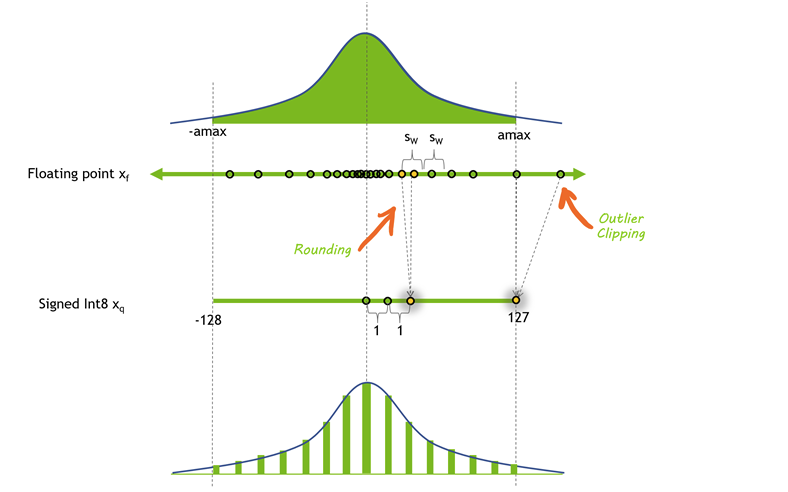
\includegraphics[width=0.8\textwidth]{quantization-value-distribution.png}
    \caption{The distribution of values before and after one possible method of quantization}
\end{figure*}

量化是减少模型权重和激活精度的过程。大多数模型以32位或16位精度进行训练,每个参数和激活元素占用32或16位内存,即单精度浮点数。然而,大多数深度学习模型可以有效地用每个值8位甚至更少来表示。

图9展示了量化前后值的分布。在这种情况下,一些精度由于舍入而丢失,一些动态范围由于裁剪而丢失,使得这些值可以用更小的格式来表示。


减少模型精度可以带来多重益处。如果模型在内存中占用更少的空间,可以在相同的硬件上容纳更大的模型。量化还意味着可以通过相同的带宽传输更多参数,这有助于加速受带宽限制的模型。

对于LLM来说,有许多量化技术涉及减少激活、权重或两者的精度。量化权重更为简单,因为它们在训练后是固定的。然而,激活值通常包含异常值,这增加了它们的动态范围,使得以低于权重的精度表示这些值变得更具挑战性。

一种选择是在模型中通过代表性数据集找到可能出现异常值的位置,并选择某些激活值使用更高的精度(如LLM.int8())。另一种选择是借用容易量化的权重的动态范围,并在激活中重复使用该范围。


\end{document}
